\begin{figure}[h]
    \centering
    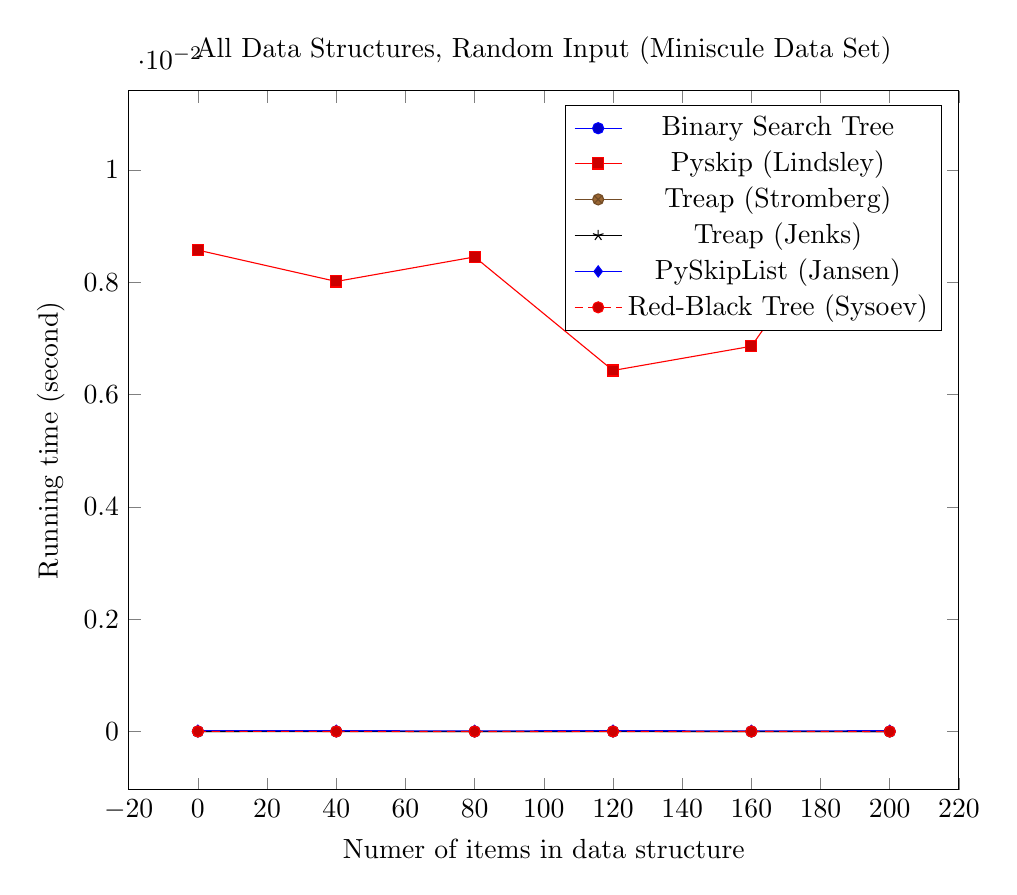
\begin{tikzpicture}
        \begin{axis}[
            xlabel={Numer of items in data structure},
            ylabel={Running time (second)},
            title={All Data Structures, Random Input (Miniscule Data Set)},
            width=\textwidth
        ]
		\addplot coordinates {
			(0, 5.752448931950483e-06)
			(40, 6.384917139090618e-06)
			(80, 5.782566465573069e-06)
			(120, 5.903036600329869e-06)
			(160, 5.903036600329869e-06)
			(200, 5.752448931950483e-06)
		};
		\addplot coordinates {
			(0, 0.008571721141755705)
			(40, 0.008013763712889598)
			(80, 0.00845046795117943)
			(120, 0.006429460971441081)
			(160, 0.00686056334846743)
			(200, 0.010367629674805912)
		};
		\addplot coordinates {
			(0, 5.391038527946534e-06)
			(40, 6.655974942226805e-06)
			(80, 4.969393056519777e-06)
			(120, 6.113859336132066e-06)
			(160, 5.119980724721529e-06)
			(200, 4.51763005120398e-06)
		};
		\addplot coordinates {
			(0, 2.7406955643627383e-06)
			(40, 2.3190500929359813e-06)
			(80, 2.1383448910228252e-06)
			(120, 2.3190500931136173e-06)
			(160, 2.1082273573114206e-06)
			(200, 2.1383448910228252e-06)
		};
		\addplot coordinates {
			(0, 1.9787219624589625e-05)
			(40, 1.8371695541929967e-05)
			(80, 1.587194024672556e-05)
			(120, 1.9004163748981283e-05)
			(160, 1.5600882443678188e-05)
			(200, 1.7950050070325574e-05)
		};
		\addplot coordinates {
			(0, 6.655974942226805e-06)
			(40, 5.631978797104864e-06)
			(80, 5.300685926812321e-06)
			(120, 5.722331398239078e-06)
			(160, 5.601861263571095e-06)
			(200, 5.391038527768899e-06)
		};
        \legend{Binary Search Tree, Pyskip (Lindsley), Treap (Stromberg), Treap (Jenks), PySkipList (Jansen), Red-Black Tree (Sysoev)}
        \end{axis}
    \end{tikzpicture}
    \caption{Average of 10 operations, benchmarked every 40, starting at 0.}
\end{figure}